%!TeX root=../tese.tex
%(dica para o editor de texto: este arquivo é parte de um documento maior)
% para saber mais: https://tex.stackexchange.com/q/78101/183146

\chapter{Perceptron multi-camadas}
\label{cap:perceptron}

Neste capítulo é descrita a implementação e funcionamento de uma versão do algoritmo \eng{perceptron}, feito a partir de um núcleo básico disponibilizado no livro de Kopec \citep{classic}, e a partir do qual foram feitas modificações e criação de novos métodos de treinamento, de validação e de avaliação do treinamento.

O perceptron aqui implementado tem o objetivo de ser utilizado muito mais para fins didáticos do que práticos e pode ser usado para tarefas de aprendizagem contanto que sejam problemas que envolvam bases de dados de tamanho pequeno ou mediano, e neste capítulo são apresentados exemplos de aplicações de classificações.

Na última parte desse capítulo é mostrado um panorama atual de implementação e uso das redes neurais, que está muito mais avançado do que esta versão simples do \emph{perceptron} que possui muitos problemas, que surgem quando tentamos treiná-lo com bases de dados maiores, que precisariam de muitos neurônios de entrada, muitas camadas ocultas e assim por diante.

\section{Derivação matemática do algoritmo de retropropagação}

Para a aprendizagem supervisionada foi utilizado o algoritmo de retropropagação (\eng{retropropagation}), que consiste na minimização de uma função de custos, a partir do gradiente, ou seja, da derivada desta função de custos, neste caso o erro quadrático médio, conforme foi definido no capítulo anterior.

De acordo com Kopec \citep{classic}, o perceptron consiste de uma rede cujo sinal, ou seja, os dados, se propagam em uma só direção, da camada de entrada para a camada de saída, passando pelas camadas ocultas uma a uma, e por isso o nome de rede \eng{feedforward} ao perceptron. Por sua vez, o erro que determinamos na camada final propaga-se no caminho inverso, sendo distribuídas correções da saída para a entrada, afetando aqueles neurônios que foram mais responsáveis pelo erro total. Por isso o nome de retropropagação.

Estendendo as definições já usadas no capítulo anterior, segue a derivação matemática do algoritmo de retropropagação. Como ficará claro mais à frente, podemos derivar as contas para apenas um neurônio por camada sem perda de generalidade. Dessa forma, se temos uma rede com $L$ camadas, o erro quadrático para um neurônio da camada de saída (a camada $L$) será:
\[
C_0 = (a^{(L)} - y)^2
\]
onde $y$ é a saída esperada, e $a^{(L)}$ é a saída de um neurônio da camada de saída.

Temos que $C_0$ é uma função de $a^{(L)}$, uma vez que $y$ é um valor fixo conhecido. Por sua vez, temos que de modo geral a saída de um neurônio é uma função do tipo:
\[
a^{(L)} = \sigma(w^{(L)}~a^{(L-1)} + b^{(L)})
\]
onde escrevemos $a^{(L-1)}$ é a saída do neurônio da camada anterior, $w^{(L)}$ é o \defi{peso} atribuido a essa saída, o que seria o parâmetro angular $A$ na Figura \ref{fig:neuronio}, e $b^{(L)}$ é o chamado \defi{viés} desse neurônio, análogo ao parâmetro linear de uma reta. Por fim temos a \defi{função de ativação} que escrevemos como $\sigma$ que é aplicada à essa equação linear.

Nota-se que internamente à função de ativação, um neurônio se comporta como uma transformação linear dos neurônios da camada anterior. Caso tivéssemos $n$ neurônios na camada anterior à de saída, teríamos então $n$ pesos, denotados com índice $i$ dessa forma: $\{ w_i^{(L)} \}_{i=1}^n$. Cabe assim à função de ativação, dar o comportamento não-linear à rede perceptron.

Como o objetivo é minimizar $C_0$, temos que calcular a influência dos pesos e dos viéses nesse custo. Já sabemos que isso será obtido com o gradiente, isto é, a derivada dessa função em relação a esses parâmetros que, são os únicos que podemos otimizar. De forma mais clara, temos que no início do treinamento da rede, atribuímos valores aleatórios aos pesos e aos viéses, e então executamos o \eng{feedforward}, de forma que a rede irá calcular sequencialmente os valores de saída em todas as suas camadas, obtidos a partir dos dados de entrada, que serão fixos, e desses parâmetros inicialmente aleatórios. A partir daí, poderemos otimizar esses parâmetros, exatamente da forma que estamos construindo.

O cálculo dessas derivadas é feito segundo a regra da cadeia, e adicionalmente iremos denotar a transformação linear interna à função de ativação por $z^{(L)} = w^{(L)}~a^{(L-1)} + b^{(L)}$, de forma que $a^{(L)} = \sigma(z^{(L)})$. Assim, ficamos com as derivadas para a camada de saída:

\begin{equation}\label{retro:1}
\frac{\del C_0}{\del w^{(L)}} = \frac{\del z^{(L)}}{\del w^{(L)}} \frac{\del a^{(L)}}{\del z^{(L)}} \frac{\del C_0}{\del a^{(L)}}
\end{equation}

\begin{equation}\label{retro:2}
\frac{\del C_0}{\del b^{(L)}} = \frac{\del z^{(L)}}{\del b^{(L)}} \frac{\del a^{(L)}}{\del z^{(L)}} \frac{\del C_0}{\del a^{(L)}}
\end{equation}

Para a camada de saída, podemos calcular diretamente cada termo dessas derivadas:

\begin{equation}\label{retro:4}
\frac{\del C_0}{\del a^{(L)}} = 2(a^{(L)} - y) ~\propto~ (a^{(L)} - y)
\end{equation}

\begin{equation}\label{retro:5}
\frac{\del a^{(L)}}{\del z^{(L)}} = \sigma^{'}(z^{(L)})
\end{equation}

\begin{equation}\label{retro:6}
\frac{\del z^{(L)}}{\del w^{(L)}} = a^{(L-1)}
\end{equation}

\begin{equation}\label{retro:7}
\frac{\del z^{(L)}}{\del b^{(L)}} = 1
\end{equation}

O que resulta, fazendo todas as substituições, em:

\begin{equation}\label{retro:10}
\frac{\del C_0}{\del w^{(L)}} = a^{(L-1)}~ \sigma^{'}(z^{(L)})~ (a^{(L)} - y)
\end{equation}

\begin{equation}\label{retro:11}
\frac{\del C_0}{\del b^{(L)}} = \sigma^{'}(z^{(L)})~ (a^{(L)} - y)
\end{equation}

Na equação \ref{retro:4} ocultamos o termo constante $2$ sob um símbolo de proporção, que a seguir iremos também ocultar, uma vez que usaremos o algoritmo do gradiente descendente, e assim, em seu lugar, e na verdade, todas as derivadas aqui mostradas serão multiplicadas pelo termo $\eta$, a \defi{taxa de aprendizagem}, conforme explicado no capítulo anterior. 

Analogamente, podemos pensar numa forma de fazer esses cálculos para as camadas ocultas. A princípio, podemos calcular:

\begin{equation}\label{retro:3}
\frac{\del C_0}{\del a^{(L-1)}} = \frac{\del z^{(L)}}{\del a^{(L-1)}} \frac{\del a^{(L)}}{\del z^{(L)}} \frac{\del C_0}{\del a^{(L)}}
\end{equation}

Usando o fato de que:

\begin{equation}\label{retro:8}
\frac{\del z^{(L)}}{\del a^{(L-1)}} = w^{(L)}
\end{equation}

Agora, seja a $i$-ésima camada oculta tal que $1 < i < L$, se observarmos a equação \ref{retro:3}, e fizermos $i = L-1$, usando a equação \ref{retro:8}, ficamos com:

\begin{equation}\label{retro:9}
\frac{\del C_0}{\del a^{(i)}} = w^{(i+1)} \frac{\del a^{(i+1)}}{\del z^{(i+1)}} \frac{\del C_0}{\del a^{(i+1)}}
\end{equation}

Podemos observar que há um mesmo termo duplo que aparece tanto nas equações \ref{retro:1} e \ref{retro:2} quanto na equação \ref{retro:9} acima, de forma que apenas o índice da camada é diferente. Para simplificar podemos nomear esse termo de \emph{delta da camada $i$}:

\begin{equation}\label{retro:12}
\Delta^{(i)} = \dfrac{\del a^{(i)}}{\del z^{(i)}} \dfrac{\del C_0}{\del a^{(i)}}
\end{equation}

Simplificando todas as demais expressões usando essa definição, ficamos com:

\begin{equation}\label{retro:13}
\frac{\del C_0}{\del w^{(i)}} = a^{(i-1)} \Delta^{(i)}
\end{equation}

\begin{equation}\label{retro:14}
\frac{\del C_0}{\del b^{(i)}} = \Delta^{(i)}
\end{equation}

Como vemos, as derivadas que precisamos todas dependem desse termo $\Delta$, que por sua vez depende do cálculo do termo $\dfrac{\del C_0}{\del a^{(i)}}$ que será calculado de 2 formas distintas:

\[ \dfrac{\del C_0}{\del a^{(i)}} = w^{(i+1)}~ \Delta^{(i+1)}  \;\;\Rightarrow \]
\begin{equation}\label{retro:15}
\Delta^{(i)} = \sigma^{'}(z^{(i)})~ w^{(i+1)}~ \Delta^{(i+1)}
\end{equation}
para as camadas ocultas.


\[ \dfrac{\del C_0}{\del a^{(L)}} = (y - a^{(L)}) \;\;\Rightarrow \]
\begin{equation}\label{retro:16}
\Delta^{(L)} = \sigma^{'}(z^{(L)})~ (y - a^{(L)})
\end{equation}
para a camada de saída.

Percebe-se a natureza recursiva do algoritmo, onde o caso base é calculado na camada de saída, e que o cálculo vai propagando-se para as camadas ocultas, em direção à camada de entrada. Por essa mesma razão, pudemos derivar as contas para uma camada, e no fim elas estão prontas pra serem implementadas para qualquer número de camadas ocultas. 

Outro fato útil é que a expressão interna do neurônio é uma transformação linear, assim as contas podem ser facilmente ajustadas para o caso geral em que há $n_i$ neurônios em dada camada $i$ da rede, conforme já explicado, e que será detalhado diretamente nos trechos de código que serão mostrados a seguir na implementação propriamente dita.

\section{Implementação do algoritmo de retropropagação}

A implementação seguiu uma estrutura orientada a objetos, voltemos então à representação visual da rede perceptron, a partir da imagem \ref{fig:estrutura_rn}. Cada círculo representa um neurônio, cada coluna vertical de neurônios é uma camada da rede, uma das camadas, a camada oculta nesse caso, está destacada em roxo na imagem. As setas representam as conexões entre as camadas de neurônios, cada neurônio de uma camada está ligado a todos os neurônios da camada anterior, o sentido dessa conexão é da esquerda pra direita, o que indica o processo de \eng{feedforward} da rede.

\begin{figure}[htb]
\centering
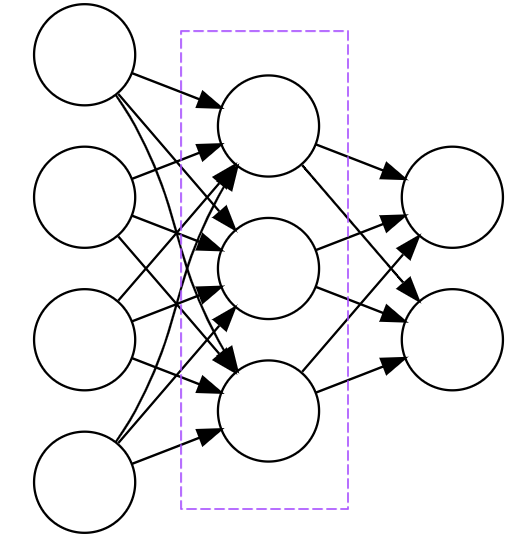
\includegraphics[width=6cm]{figuras/estrutura_rn}
\caption{Visão estrutural da rede perceptron. A linha tracejada destaca uma das camadas da rede.}
\label{fig:estrutura_rn}
\end{figure}

A implementação do perceptron deste trabalho teve como base a implementação feita por Kopec \citep{classic}, a partir da qual foram adicionados outros recursos, como o viés dos neurônios, não presentes na implementação de Kopec, como o uso da biblioteca \emph{Numpy} para o uso de seus métodos mais eficientes para lidar com listas de números de ponto flutuante. Além dessa base, também estão implementadas várias outras classes, que serão explicadas de modo mais geral.

\subsection{O neurônio}

O primeiro passo é implementar a classe \emph{Neuron} para representar cada neurônio. Esta é uma classe de entidade bem simples, contendo apenas um construtor, e o método \eng{output} que recebe os valores de entrada para esse neurônio e faz o cálculo da transformação linear e a seguir aplica e retorna o valor da função de ativação utilizada, que é passada como parâmetro ao construtor da classe. A listagem \ref{lst:neuron} abaixo mostra este método, em conjunto com o construtor da classe.

\begin{scriptsize}
\estiloR
\begin{lstlisting}[caption={Trecho da classe Neuron}, label={lst:neuron}, escapeinside={\%}]
class Neuron:
    def __init__(self, weights, bias, learning_rate, ativacao, der_ativacao):
        '''(list[float], float, float, Callable, Callable) -> None'''
        ...

    def output(self, inputs):
        '''(list[float]) -> float'''
        self.output_cache = np.dot(inputs, self.weights) + self.bias
        return self.ativacao(self.output_cache)
\end{lstlisting}
\end{scriptsize}

A função \emph{np.dot} da biblioteca \emph{Numpy} é utilizada para calcular o produto escalar entre os valores de entrada e os pesos desse neurônio. O valor da transformação linear é armazenado num atributo de classe antes da aplicação da função de ativação, pois será utilizado mais à frente durante o treinamento da rede.

\subsection{A função de ativação}

A função de ativação possui o papel de ativar ou não a saída de um neurônio, conforme visto no capítulo anterior, e a forma com que essa ativação ocorre é definida pela função utilizada. Aqui o termo \emph{ativar} significa que a função irá retornar um valor mais próximo de $1$ enquanto que uma não-ativação retornará um valor mais próximo de $0$. Essa é uma restrição para a função de ativação para a camada de saída, que será sempre da forma:

\[ f: \mathbb{R} \rightarrow [0, 1] \]

No caso do neurônio biológico, quando dizemos que ele ativa/transmite ou não o sinal elétrico que chegou até ele, é como se ele \emph{retornasse} apenas $0$ ou $1$. De fato, poderíamos até usar uma função similar a essa em alguma camada de nossa rede artificial, e este tipo de função escada tem a seguinte definição:

\[
f(x) = 
\left\{
\begin{array}{lcr}
1 & \text{se} & x \geq 0\\
0 & \text{se} & x < 0
\end{array}
\right.
\]

A utilização dessa função de ativação, conforme nos diz Grus \citep{data}, faria com que um neurônio fizesse simplesmente a distinção entre espaços separados pelo hiperplano de pontos tal que $ <w.x> + b = 0$, ou seja, o hiperplano definido pelos pontos de entrada cuja transformação linear resultasse em zero.

Esta função é claramente não contínua e portanto não diferenciável, e precisamos de uma função de ativação que o seja, uma vez que algumas das equações da otimização que calculamos anteriormente, dependem da expressão de sua derivada. É por essa razão, que Grus \citep{data} nos explica que passou-se a considerar uma aproximação suave da função escada, essa aproximação é a função \eng{sigmoid}:

\[
\sigma(x) = \frac{1}{1 + e^{-x}}
\]

Ela retorna valores somente no intervalo $[0, 1]$, igualmente à função escada, sua inspiração. Essa característica, no entanto, não é uma restrição para as camadas ocultas da mesma forma que é para a camada de saída, uma vez apenas a camada de saída será comparada com valores esperados no intervalo $[0, 1]$. A sua derivada pode ser facilmente calculada, e sua expressão simplifica-se como:

\[
\sigma^{'}(x) = \sigma(x)(1-\sigma(x))
\]

Podemos comparar o comportamento dessas funções de ativação no gráfico presente na imagem \ref{fig:ativacao} abaixo. A seguir, na listagem \ref{lst:ativacao}, um trecho do script \texttt{util.py} com a implementação da função \eng{sigmoid} e de sua derivada.

\newpage

\begin{figure}[htb]
\centering
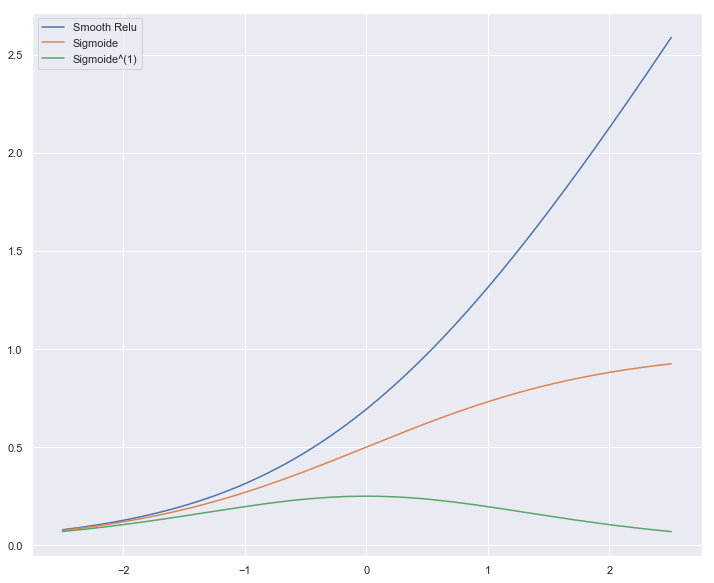
\includegraphics[width=12cm]{figuras/ativacao}
\caption{Comparação entre as funções de ativação do tipo escada e a \eng{sigmoid}.}
\label{fig:ativacao}
\end{figure}

\begin{scriptsize}
\estiloR
\begin{lstlisting}[caption={Trecho do script util.py}, label={lst:ativacao}, escapeinside={\%}]
def sigmoid(x):
    '''(float) -> float'''
    return 1.0 / (1.0 + np.exp(-x))

def der_sigmoid(x):
    '''(float) -> float'''
    sig = sigmoid(x)
    return sig * (1 - sig)
\end{lstlisting}
\end{scriptsize}

Com a popularização das redes neurais, várias outras funções de ativação foram criadas para ativarem as camadas ocultas do treinamento, devido aos problemas que podem acontecer ao se utilizar função \eng{sigmoid}. Podemos identificar um desses problemas analisando seu gráfico. Vemos que ela se aproxima de $1$, que é a ativação máxima, rapidamente a partir de $x > 4$, e aproxima-se simetricamente de zero com valores a partir de $x < -4$. 

Como o método do gradiente tenta ajustar os valores dos pesos a partir dos valores de saída e esses ajustes dependem da derivada da função de ativação, temos que levar em conta o comportamento da derivada da função \eng{sigmoid}, o qual podemos observar a partir de seu gráfico na figura \ref{fig:der_sigm}.

\begin{figure}[htb]
\centering
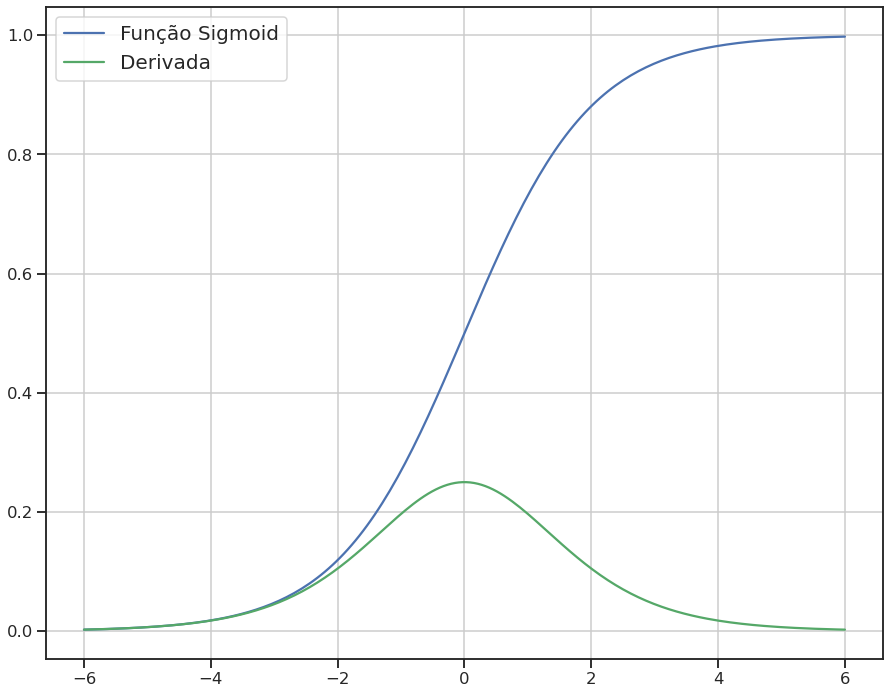
\includegraphics[width=12cm]{figuras/der_sigm}
\caption{Gráficos da função \eng{sigmoid} e sua derivada.}
\label{fig:der_sigm}
\end{figure}

Como podemos ver, a derivada retorna valores sempre menores do que $1$, e além disso aproxima-se de $0$ tão rapidamente quanto a \eng{sigmoid} aproxima-se de $1$. Isso faz com que atualizações para valores de saída que já estão muito altos não sejam efetivos para diminuí-los, pois justamente nessa região a derivada está muito próxima de $0$. Essa é a desvantagem da função \eng{sigmoid}.

Um problema relacionado a este é que se a regra da cadeia em \ref{retro:1} e \ref{retro:2}, com as derivadas da função de ativação dadas em \ref{retro:5} multiplicadas através das várias camadas, pode resultar num número muito grande, se todas as derivadas resultarem em valores maiores do que $0$, ou resultar num número muito próximo de $0$ se todas as derivadas forem menores do que $0$. Isto faz com que atualizações dadas pelo gradiente sejam instáveis. Este é o problema descrito por Matheus Facure \citep{matheus_2} e nomeado como problema do gradiente explodindo/desvanecendo. (\eng{exploding/vanishing gradient problem}).

Assim, conforme nos diz Facure \citep{matheus}, a utilização da função \eng{sigmoid} não é mais recomendada em problemas que envolvam de redes neurais maiores, sendo bem comum o problema do gradiente explodindo, já que a derivada é sempre maior do que $0$. Porém, ele também diz que alguns modelos probabilísticos de variáveis binárias, modelagem de problemas biológicos onde ela é uma aproximação mais plausível da ativação elétrica-biológica, e também alguns modelos não supervisionados de redes tem restrições que fazem com que seja não só desejável como também necessário o uso da função \eng{sigmoid}.

A próxima função de ativação é a o tangente hiperbólico $\tanh(x)$, ela é similar à \eng{sigmoid} e pode ser escrita em função dela. Ela retorna valores no intervalo $[-1, 1]$ mas sua derivada retorna valores mais próximos de $1$, chegando ao valor máximo de $1$ quando $x = 0$. A expressão em função da função \eng{sigmoid} e a derivada da função tangente hiperbólica são dadas por:

\[ tanh(x)=2\sigma(2x) - 1   \quad \quad  tanh'(x)=1 - tanh^2(x) \]

Na figura \ref{fig:tanh} podemos ver o gráfico da função e de sua derivada, a partir do que podemos notar como a derivada da \emph{tanh} retorna valores maiores do que a derivada da função \eng{sigmoid}.

\begin{figure}[htb]
\centering
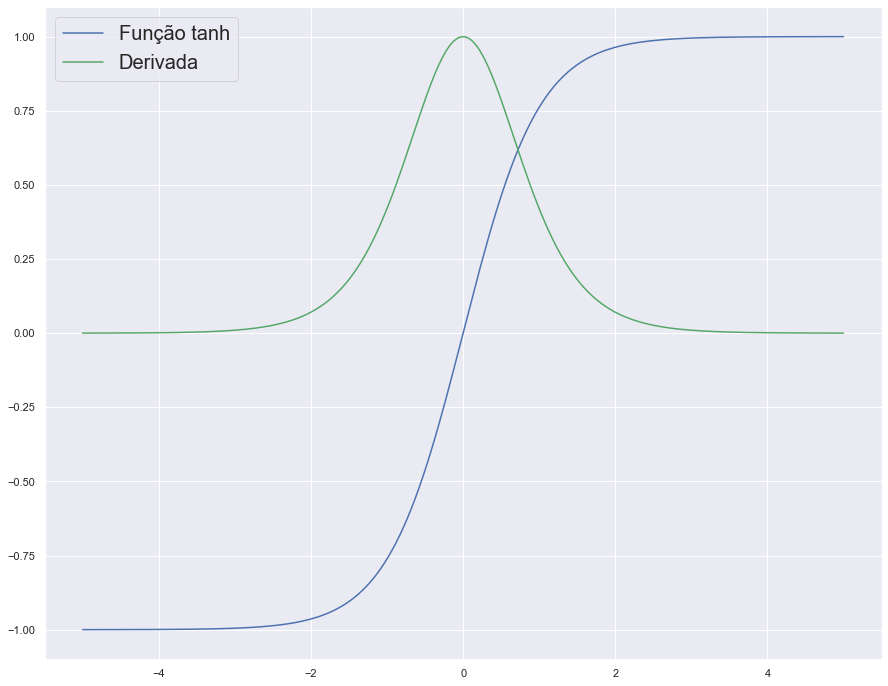
\includegraphics[width=12cm]{figuras/tanh}
\caption{Gráficos da função tangente hiperbólico e sua derivada.}
\label{fig:tanh}
\end{figure}

O próximo avanço é conseguido com a função de ativação linear retificada (\defi{RELU}). Essa função é quase a função identidade, exceto que na região negativa do domínio ela vale identicamente $0$. Ela não é derivável no ponto $x=0$, mas podemos estender a definição fixando seu valor em $1$ nesse ponto. Sua definição e de sua derivada estendida é dada por:

\[
ReLU(x)=max\{0, x\}   \quad \quad  ReLU'(x)=
	\begin{cases}
    	1, & \text{se } x\ge 0\\
    	0, & \text{c.c.}
	\end{cases}
\]

Podemos ver seus gráficos, na figura \ref{fig:relu}, a seguir. Usar essa função de ativação torna até mesmo a execução do código mais rápida, uma vez que não há cálculos matemáticos a serem feitos, apenas uma função de máximo que é trivial. Além disso, podemos notar que a derivada se mantém com o valor $1$ constante enquanto o neurônio é ativado, sendo uma forma de tentar resolver o problema do gradiente explodindo/desvanecendo, além de agilizar o processo de treinamento. 

\begin{figure}[htb]
\centering
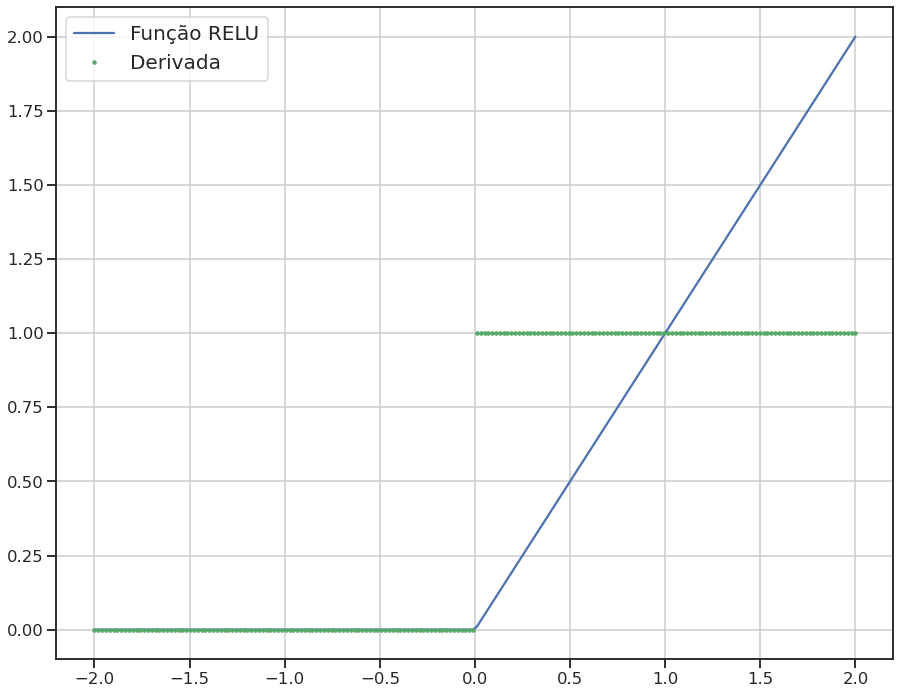
\includegraphics[width=12cm]{figuras/relu}
\caption{Gráficos da função \eng{RELU} e sua derivada.}
\label{fig:relu}
\end{figure}

Essa é a razão, conforme explica Facure \citep{matheus}, dessa função ter contribuido para o recente aumento de popularidade das redes neurais. Adicionalmente, Bing Xu \citep{xu_relu} ressalta que outra vantagem das funções do tipo \eng{RELU}, além de resolver o problema do gradiente explodindo/desvanescendo, é a de aumentar a velocidade da convergência do algoritmo de treinamento rumo a um mínimo da função de custos.

Uma desvantagem da função \eng{RELU} é a chance de neurônios serem desativados permanentemente, já que uma vez que ele zera, a função de ativação e sua derivada são ambos $0$, de forma que ele nunca mais irá aumentar durante o treinamento, tornando-se neurônios \emph{mortos}.

O próximo avanço foi dado pela função conhecida como \eng{Leaky RELU}. Quase identica à \eng{RELU}, exceto que na parte negativa do domínio ao invés de $0$ a função retorna $x/\alpha$, onde $\alpha \in (0, \infty)$. Isso já imediatamente corrige o problema dos neurônios desativados. A definição da função e de sua derivada, dada por Xu \citep{xu_relu}, é:

\[
LeakyReLU(x, \alpha) = 
\begin{cases}
    	x, & \text{se } x\ge 0\\
    	x/\alpha, & \text{c.c.}
	\end{cases}
\quad \quad  
LeakyReLU'(x, \alpha) =
	\begin{cases}
    	1, & \text{se } x\ge 0\\
    	\alpha, & \text{c.c.}
	\end{cases}
\]

A partir dos resultados dos estudos feitos por Xu \citep{xu_relu}, a função \eng{Leaky RELU}, e suas variações, se saíram consistentemente melhores do que a \eng{RELU} para as bases de dados de pequeno e médio portes. Além disso, ele testou a performance para diferentes valores de $\alpha$, obtendo os melhores resultados com $\alpha = 5.5$. Este parâmetro é conhecido como \defi{vazamento}, que dá o nome à função. Podemos ver o seu comportamento no gráfico da imagem \ref{fig:l_relu}.

\begin{figure}[htb]
\centering
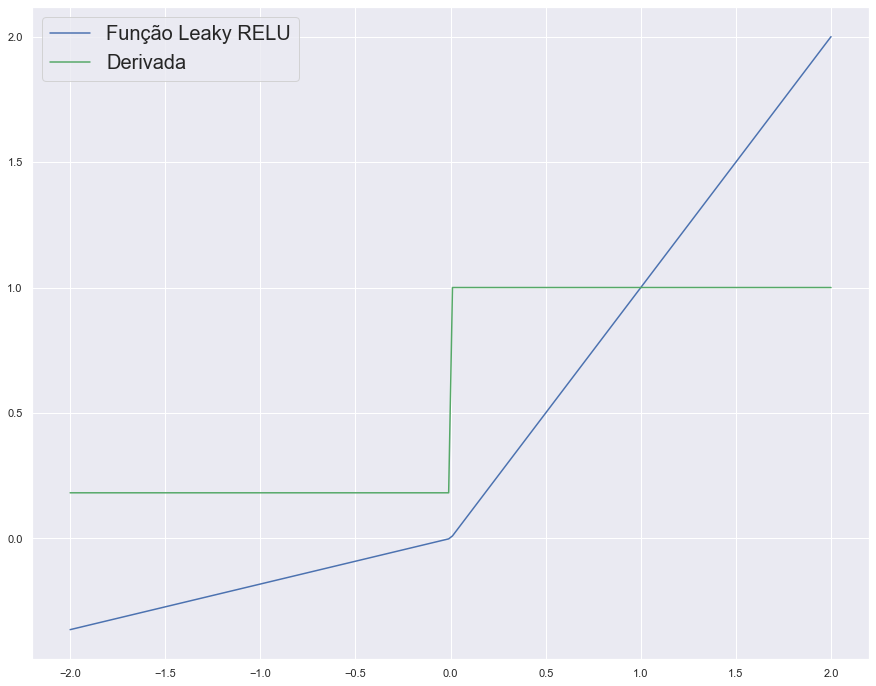
\includegraphics[width=12cm]{figuras/l_relu}
\caption{Gráficos da função \eng{Leaky RELU} e sua derivada.}
\label{fig:l_relu}
\end{figure}

Por fim, temos a função de unidade linear exponencial \eng{ELU}, proposta por Djork-Arné Clevert \citep{clevert}, que é definida, com $\alpha > 0$, por:

\[
ELU(x, \alpha)=
	\begin{cases}
    	x, & \text{se } x\ge 0\\
    	\alpha(e^x - 1), & \text{c.c.}
	\end{cases}
\quad \quad
ELU'(x, \alpha)=
	\begin{cases}
    	1, & \text{se } x\ge 0\\
    	ELU(x, \alpha)+\alpha, & \text{c.c.}
	\end{cases} 
\]

Em seu artigo, Clevert \citep{clevert} utiliza o valor $\alpha = 1$, e com a função \eng{ELU} conseguiu perfomances melhores, tanto de resultados mais corretos, quanto de velocidade de treinamento, em relação às funções \eng{RELU} e \eng{Leaky RELU} para as mesmas bases de dados avaliadas por XU \citep{xu_relu}, mesmo com o uso da função exponencial em sua definição o que em teoria deveria diminuir a performance do treinamento. Podemos observar o comportamento dessa função e de sua derivada, com $\alpha = 1$ no gráfico mostrado na figura \ref{fig:elu}.

\begin{figure}[htb]
\centering
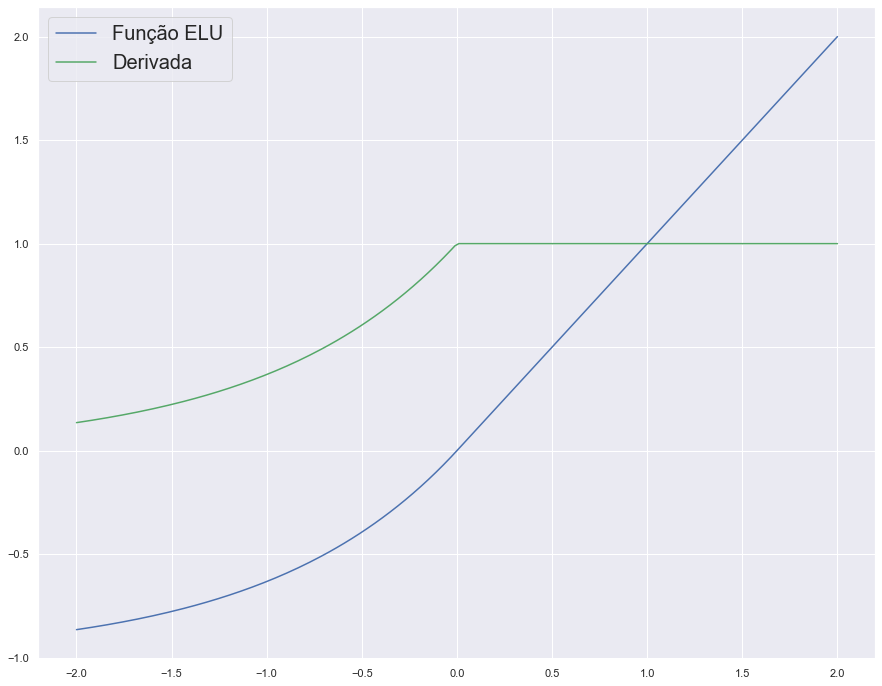
\includegraphics[width=12cm]{figuras/elu}
\caption{Gráficos da função \eng{ELU} e sua derivada.}
\label{fig:elu}
\end{figure}

Testes feitos em condições similares por Facure \citep{matheus}, mostram que essa diferença não é tão significativa em relação à \eng{Leaky RELU}, mas que ambas, \eng{Leaky RELU} e a \eng{ELU} são sim melhores do que a original \eng{RELU}, o que é consistente com o fato delas resolverem teoricamente as desvantagens dela. E são todas obviamente melhores escolhas do que a função \eng{sigmoid}, em todos os estudos acima citados.

Na prática, podemos testar qual função de ativação irá performar melhor para o problema que queremos resolver. A abordagem mais comum, conforme descrita por Facure \citep{matheus} é utilizar a função \eng{Leaky RELU} nas camadas ocultas, sendo o modo mais simples de obtermos bons resultados graças ao seu comportamento. Podemos avaliar a utilização das outras de acordo com o problema em questão, dado que algumas funções se saem melhor em alguns contextos específicos como é o caso da função \eng{sigmoid}.

\subsection{As camadas}

A classe \emph{Layer} representa uma camada de neurônios. Cada camada conecta-se com a sua camada anterior, com exceção da camada de entrada. Por essa razão, a rede perceptron possui um sentido único de conexão, que vai da entrada para a saída, passando por cada camada oculta. A classe é constituída de uma lista de objetos da classe \emph{Neuron}, uma referência à camada anterior e uma lista para armazenar as saídas dos seus neurônios.

O construtor de \emph{Layer} é responsável por inicializar seus neurônios. Nessa implementação todos os neurônios de uma camada irão usar a mesma função de ativação e a mesma taxa de aprendizagem. Além de receber esses parâmetros, o número de neurônios dessa camada, e a referência da camada anterior, o construtor inicializa os pesos de cada neurônio, lembrando que cada neurônio de uma camada possui a mesma quantidade de pesos do que a quantidade de neurônios da camada anterior, e também inicializa o viés de cada neurônio. 

Na listagem \ref{lst:layer_1} está o trecho do construtor que inicializa os pesos dos neurônios. Se a camada que estamos inicializando é a camada de entrada, então não criamos pesos e o viés, pois os valores de entrada serão utilizados diretamente como a saída dessa camada, este é o teste presente na linha 11 da listagem, pois a camada de entrada não possui referência a uma camada anterior já que ela é a primeira camada da rede.

A linha 12 de \ref{lst:layer_1} inicializa os pesos dos neurônios da camada. Para fazer isso utiliza uma função que está definida no script \texttt{util.py}, que sortea números aleatórios para esses pesos seguindo uma distribuição normal de média $0$ e desvio-padrão $0.3$ e além disso \emph{truncada} no intervalo $[-1, 1]$, para que nenhum peso esteja fora desse domínio e para que em média esse valor seja $0$. O viés é inicializado com um valor constante, próximo de zero, nesse caso com $0.01$.

\begin{scriptsize}
\estiloR
\begin{lstlisting}[caption={Trecho da classe \eng{Layer}}, label={lst:layer_1}, escapeinside={\%}]
class Layer:
    def __init__(self, previous_layer, num_neurons, learning_rate,
                 ativacao=None, der_ativacao=None):
        '''(Layer, int, float, Callable, Callable) -> None
        Construtor da Camada de Neurônios
        '''
        ...
        for i in range(num_neurons):
            pesos = None
            bias = None
            if previous_layer is not None:
                pesos = normal_t.rvs(len(previous_layer.neurons))
                bias = 0.01
            
            neuron = Neuron(pesos, bias, learning_rate, ativacao, der_ativacao)
            self.neurons = np.append(self.neurons, neuron)
\end{lstlisting}
\end{scriptsize}

Este procedimento é usado para tentar mitigar dois problemas que podem acontecer, conforme explicado por James Dellinger \citep{layers_1}. Se inicializarmos os pesos com muitos números não tão próximos de $0$, numa rede como muitos neurônios e muitas camadas, esses pesos podem somar-se rapidamente através das camadas, resultando em números com valores absolutos muito grandes na camada de saída o que pode prejudicar o treinamento e aprendizado da rede.

Se pelo contrário, inicializarmos todos os pesos com números muito próximos de $0$, ocorre o problema oposto, os neurônios tem seus valores zerados, tornando-se \emph{neurônios desativados}, que se tornam inúteis para o aprendizado já que serão ignorados durante o restante do treinamento. 

Dellinger \citep{layers_1} distute esses problemas no contexto de redes bem grandes, com mais de $100$ camadas, e exibe sua solução heurística que é utilizar uma distribuição normal (não-truncada) com média $0$ e com desvio-padrão $\sqrt{2/n}$, sendo $n$ o número de neurônios da camada anterior.

Para nossos fins didáticos, testei alguns desvios-padrão como $1$, $0.3$ e $0.1$, em um dos exemplos que serão mostrados ainda nesse capítulo, e dentre eles, o valor $0.3$ se saiu melhor sendo o suficiente para não explodir e nem desativar os neurônios da única camada oculta que foi usada na aplicação-exemplo em questão.

O desvio-padrão de $0.3$ auxilia na tarefa de restringir os valores no intervalo $[-1, 1]$, sem que precisemos truncar muitos valores o que poderia aumentar a massa de probabilidade dos extremos $-1$ e $1$, já que valores mais distantes da média do que $3$ vezes o desvio-padrão são raramentes obtidos de uma distribuição normal. 

Após inicializar cada neurônio, salvamos ele na lista de neurônios dessa camada, que é um dos atributos de classe discutidos no primeiro parágrafo. A próxima tarefa de uma camada é processar as entradas recebidas e retornar as saídas. Podemos observar esse comportamento na listagem \ref{lst:layer_2}.

\newpage

\begin{scriptsize}
\estiloR
\begin{lstlisting}[caption={Trecho da classe \eng{Layer}}, label={lst:layer_2}, escapeinside={\%}]
def outputs(self, inputs):
        '''(list[float]) -> list[float]
        Armazena em cache as saidas dos neuronios e a retornam
        Se for uma camada de entrada, usa elas diretamente
        '''
        if self.previous_layer is None:
            self.output_cache = inputs
        else:
            self.output_cache = np.array([n.output(inputs) for n in self.neurons])
        return self.output_cache
\end{lstlisting}
\end{scriptsize}

A camada de entrada não processa os dados, usando-os diretamente. As demais camadas devem processar cada neurônio, usando seu próprio método de processamento, aplicando a transformação linear e em seguida a função de ativação. O resultado é armazenado numa lista \eng{numpy} que é o atributo de classe \texttt{output$\_$cache}, que armazena as saídas dessa camada para uso posterior; por fim, a lista das saídas da camada é retornada.

A última tarefa da classe \eng{Layer} é calcular os termos $\Delta$ definidos pelas equações \ref{retro:15} e \ref{retro:16}, que definem respectivamente o cálculo que é feito se estamos calculando as derivadas para as camadas ocultas e o cálculo feito para a camada de saída. As duas versões são exibidas na listagem \ref{lst:layer_3} abaixo.

\begin{scriptsize}
\estiloR
\begin{lstlisting}[caption={Trecho da classe \eng{Layer}}, label={lst:layer_3}, escapeinside={\%}]
def calcular_delta_camada_de_saida(self, expected):
        '''(list[float]) -> None'''
        for i, neuron in np.ndenumerate(self.neurons):
            der_cost = expected[i[0]] - self.output_cache[i]
            neuron.delta = neuron.der_ativacao(neuron.output_cache) * der_cost

    def calcular_delta_camada_oculta(self, next_layer):
        '''(Layer) -> None'''
        for i, neuron in np.ndenumerate(self.neurons):
            next_weights = np.array([n.weights[i[0]] for n in next_layer.neurons])
            next_deltas = np.array([n.delta for n in next_layer.neurons])
            der_cost = np.dot(next_weights, next_deltas)
            neuron.delta = neuron.der_ativacao(neuron.output_cache) * der_cost
\end{lstlisting}
\end{scriptsize}

Os algoritmos são as traduções quase literais das equações \ref{retro:15} e \ref{retro:16}. Podemos ver a natureza recursiva da regra da cadeia nas 2 linhas finais, onde usamos os deltas calculados da próxima camada para calcular os deltas da camada atual. O caso base é a função que calcula o delta da camada de saída. A lógica que orquestra essa recursão está implementada na próxima classe.

\subsection{A rede}

A classe \eng{Network} representa a rede neural como um todo. Ela armazena uma lista de camadas, ou seja, objetos do tipo \eng{Layer}, a partir dos parâmetros que recebe em seu construtor, que são a estrutura da rede que será criada, que é um vetor de inteiros que representam as quantidades de neurônios para cada camada. Além disso, recebe a taxa de aprendizado que será utilizada em toda a rede, nessa versão, e quais as funções de ativação que serão utilizadas nas camadas ocultas e na camada de saída.

A listagem \ref{lst:network_1} exibe o trecho do construtor que cria cada camada e insere na lista de camadas do objeto da classe atual. A camada de entrada não possui camada anterior, nem função de ativação. Além disso, a camada de saída pode utilizar uma função de ativação diferente daquela utilizada pelas camadas ocultas, que usarão a mesma.

\begin{scriptsize}
\estiloR
\begin{lstlisting}[caption={Trecho da classe \eng{Network}}, label={lst:network_1}, escapeinside={\%}]
class Network:
    def __init__(self, layer_structure, taxa, ativacoes):
        '''(list[int], float, Tuple[Callable]) -> None'''
        ...
        self.layers = np.array([], dtype=np.float64)
        self.estrutura = layer_structure

        # camada de entrada
        input_layer = Layer(None, self.estrutura[0], taxa)
        self.layers = np.append(self.layers, input_layer)

        # camadas oculta(s)
        for previous, qtd_neurons in np.ndenumerate(self.estrutura[1::l]):
            next_layer = Layer(self.layers[previous[0]], qtd_neurons, taxa,
                               ativacoes[0], ativacoes[1])
            self.layers = np.append(self.layers, next_layer)

        # camada de saída
        output_layer = Layer(self.layers[-1], self.estrutura[-1], taxa,
                               ativacoes[2], ativacoes[3])
        self.layers = np.append(self.layers, output_layer)
\end{lstlisting}
\end{scriptsize}

A primeira tarefa da classe Network é o de processar entradas, fazendo elas atravessarem a rede, camada a camada, até a camada de saída, e retornar as saídas obtidas. É o processo de \eng{feedforward} explicado no início do capítulo. Sua implementação mesmo para o caso geral de multi-camadas é bem simples, conforme exibido na listagem \ref{lst:network_2} abaixo.

\begin{scriptsize}
\estiloR
\begin{lstlisting}[caption={Trecho da classe \eng{Network}}, label={lst:network_2}, escapeinside={\%}]
def feedforward(self, entrada):
    '''(list[float]) -> list[float]'''
    ...
    saida = self.layers[0].outputs(entrada)
    for i in range(1, len(self.layers)):
        saida = self.layers[i].outputs(saida)
    return saida
\end{lstlisting}
\end{scriptsize}

A próxima tarefa é treinar a rede, passando uma lista de entradas e saídas esperadas, realizando o procedimento de \eng{backpropagate} para atualizar os pesos e viéses dos neurônios de cada camada, tudo isso em sequência, para cada entrada fornecida. É o que está literalmente implementado na listagem \ref{lst:network_3} abaixo.

\begin{scriptsize}
\estiloR
\begin{lstlisting}[caption={Trecho da classe \eng{Network}}, label={lst:network_3}, escapeinside={\%}]
def train(self, entradas, saidas_reais):
    '''(list[list[floats]], list[list[floats]]) -> None
    ...
    for i, xs in enumerate(entradas):
        ys = saidas_reais[i]
        _ = self.feedforward(xs)
        self.backpropagate(ys)
        self.update_weights()
        self.update_bias()
	return saida
\end{lstlisting}
\end{scriptsize}

Cada chamada à função \eng{train} significa o procedimento de treinamento sendo executado uma única vez. Cada vez que a rede é treinada dizemos que ela avançou em uma \defi{época} de treinamento. O treinamento consiste em primeiramente executar o \eng{feedforward} para uma entrada, para que as camadas possam armazenar as saídas correspondentes aos valores atuais de seus parâmetros, os pesos e viéses, assim como as saídas em seus atributos \eng{output$\_$cache}, que serão usados pelo método \eng{backpropagate} a seguir, de acordo com as equações que derivamos para o processo de treinamento.

O funcionamento do método \eng{backpropagate} pode ser visto na listagem \ref{lst:network_4} a seguir. Tudo o que ele faz aqui é calcular os deltas das camadas, na ordem correta, começando pela camada de saída, e depois percorrendo as demais camadas do final para o início da rede, fazendo a chamada para cada objeto da classe \eng{Layer} que constitui a rede.

\begin{scriptsize}
\estiloR
\begin{lstlisting}[caption={Trecho da classe \eng{Network}}, label={lst:network_4}, escapeinside={\%}]
def backpropagate(self, saidas_reais):
    '''(list[float]) -> None
    Calcula as mudanças em cada neurônio com base nos erros da saída
    em comparação com a saída esperada
    '''
    # calcula delta para os neurônios da camada de saída
    last_layer = len(self.layers) - 1
    self.layers[last_layer].calcular_delta_camada_de_saida(saidas_reais)
    
    # calcula delta para as camadas ocultas, da saída para o início da rede
    for l in range(last_layer - 1, 0, -1):
        self.layers[l].calcular_delta_camada_oculta(self.layers[l + 1])
\end{lstlisting}
\end{scriptsize}

A seguir, atualiza-se os pesos e os viéses com os métodos correspondentes, que podem ser visualizados na listagem \ref{lst:network_5}. Como os valores são todos armazenados nos atributos de estado dos neurônios e das camadas, implementamos diretamente as contas das equações que obtemos para o método do gradiente e da regra da cadeia da retroprogação. Dessa forma, o que fazemos na classe \eng{Network} é basicamente traduzir a matemática para a sintaxe da linguagem Python.

\newpage

\begin{scriptsize}
\estiloR
\begin{lstlisting}[caption={Trecho da classe \eng{Network}}, label={lst:network_5}, escapeinside={\%}]
def update_weights(self):
    '''(None) -> None'''
    ...
    for layer in self.layers[1:]: # pula a camada de entrada
        for neuron in layer.neurons:
            for w in range(len(neuron.weights)):
                neuron.weights[w,] = neuron.weights[w,] + (neuron.learning_rate
                     * (layer.previous_layer.output_cache[w]) * neuron.delta)

def update_bias(self):
    '''(None) -> None'''
    ...
    for layer in self.layers[1:]: # pula a camada de entrada
        for neuron in layer.neurons:
            neuron.bias = neuron.bias + neuron.learning_rate * neuron.delta
\end{lstlisting}
\end{scriptsize}